%%%%%%%%%%%%%%%%%%%%%%%%%%%%%%%%%%%%%%%%
%% MCM/ICM LaTeX Template %%
%% 2024 MCM/ICM           %%
%%%%%%%%%%%%%%%%%%%%%%%%%%%%%%%%%%%%%%%%
\documentclass[12pt]{article}
\usepackage{geometry}
\geometry{left=1in,right=0.75in,top=1in,bottom=1in}

%%%%%%%%%%%%%%%%%%%%%%%%%%%%%%%%%%%%%%%%
% Replace ABCDEF in the next line with your chosen problem
% and replace 1111111 with your Team Control Number
\newcommand{\Problem}{A}
\newcommand{\Team}{2403424}
%%%%%%%%%%%%%%%%%%%%%%%%%%%%%%%%%%%%%%%%

\usepackage{newtxtext}
\usepackage{amsmath,amssymb,amsthm}
\usepackage{newtxmath} % must come after amsXXX
\usepackage{cite}
\usepackage{graphicx}
\usepackage{xcolor}
\usepackage{fancyhdr}
\usepackage{listings}
\usepackage{xeCJK}
\lhead{Team \Team}
\rhead{}
\cfoot{}

\newtheorem{theorem}{Theorem}
\newtheorem{corollary}[theorem]{Corollary}
\newtheorem{lemma}[theorem]{Lemma}
\newtheorem{definition}{Definition}
%%%%%%%%%%%%%%%%%%%%%%%%%%%%%%%%
\begin{document}
\graphicspath{{.}}  % Place your graphic files in the same directory as your main document
\DeclareGraphicsExtensions{.pdf, .jpg, .tif, .png}
\thispagestyle{empty}
\vspace*{-16ex}
\centerline{\begin{tabular}{*3{c}}
		\parbox[t]{0.3\linewidth}{\begin{center}\textbf{Problem Chosen}\\ \Large \textcolor{red}{\Problem}\end{center}}
		 & \parbox[t]{0.3\linewidth}{\begin{center}\textbf{2024\\ MCM/ICM\\ Summary Sheet}\end{center}}
		 & \parbox[t]{0.3\linewidth}{\begin{center}\textbf{Team Control Number}\\ \Large \textcolor{red}{\Team}\end{center}} \\
		\hline
	\end{tabular}}
%%%%%%%%%%% Begin Summary %%%%%%%%%%%
% Enter your summary here replacing the (red) text
% Replace the text from here ...
\begin{center}
	\textbf{\Huge Lamprey: A New Model for the Spread of an Invasive Species}
	\begin{figure}[h]
		\centering
		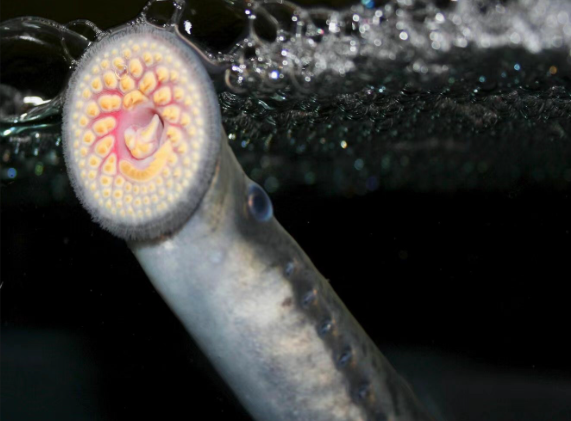
\includegraphics[width=0.7\textwidth]{LampreyFigure.png}
		\caption{Lamprey by Great Lakes Science Center\cite{sea-lamprey-2}.}
	\end{figure}
	% real summary beginning
\end{center}
As a powerful invasive species in the Great Lakes from the 1940s, lamprey populations are closely linked to the entire Great Lakes ecosystem. The female propotion of lampreys is positively correlated with the growth rate in their larval stages, and the growth rate of these larvae is affected by the amount of available food resources. The purpose of this study was to establish an analytical model to simulate the reproductive activities of lampreys under the influence of sex ratio changes and to evaluate the impact of sex ratio change mechanisms on lamprey offspring. We also build models of interactions between lampreys and other species to analyze the relationship between lamprey population development and ecosystems. \newline
In the study, we used a total of three models; \\
\textbf{Model 1}: Lotka-Volterra model that introduced gender change factors;\\
\textbf{Model 2}: Lamprey's body shape-first mate selection strategy and reproduction model;\\
\textbf{Model 3}: Based on the multi-species Lotka-Volterra model Matrix iteration model. \\We hope this study will help optimize the control of lampreys in the Great Lakes, and provide assistance in studying the reproductive activities of lamprey populations. 
% to here
%%%%%%%%%%% End Summary %%%%%%%%%%%
\newpage
\tableofcontents
\newpage
%%%%%%%%%%%%%%%%%%%%%%%%%%%%%%
\clearpage
\pagestyle{fancy}
% Uncomment the next line to generate a Table of Contents
%\tableofcontents 
\newpage
\setcounter{page}{1}
\rhead{Page \thepage\ }
%%%%%%%%%%%%%%%%%%%%%%%%%%%%%%


%%%%%%%%%%%%%%%%%%%%%%%%%%%%%%
\section{Introduction}
\subsection{Problem Background}
Sea lampreys in the Great Lakes region exhibit sex ratio variation that adapts to environmental conditions. 
The Great Lakes ecosystem has observed fluctuations in lamprey populations, with the sex ratio influenced by 
the growth rates during their larval phase, which are contingent upon food availability. In environments with 
limited food, a slower growth rate skews the population toward a higher male ratio up to 78\%. Conversely, with 
better food availability, the male percentage decreases to approximately 56\%. The sex ratio adaptation in sea 
lampreys affects prey species, predator populations, and competition dynamics within the Great Lakes. The ability 
to adjust sex ratios allows lampreys to potentially stabilize their population in varying conditions, influencing 
the broader ecosystem balance.
\subsection{Restatement of the Problem}
• What is the impact on the larger ecological system when the population of lampreys\\
 can alter its sex ratio?\\
• What are the advantages and disadvantages to the population of lampreys?\\
• What is the impact on the stability of the ecosystem given the changes in the sex ratios of lampreys?\\
• Can an ecosystem with variable sex ratios in the lamprey population offer advantages to others in the ecosystem, such as parasites?\\
\section{Approach to Problem Solving}
\subsection{Q1}
为了研究七鳃鳗性比变化的能力对更大的生态系统的影响,我们引入了 Lotka-Votterra 模型(在五大湖,七鳃鳗的生活环境十分优越,基本没有天敌,其相关的关系主要为捕食与竞争,故可以使用 Lotka-Votterra 模型)。此处更大可做两种解释,一种是七鳃鳗以外的五大湖物种,另一个可以涵盖更宏观的生态系统,比如大西洋。根据 Lotka-Volterra Competition Models我们改良了模型的系数,并引入了性比因子来解释种群数量。 

       模型中的N2物种实际上并非是某一特定物种,而是七鳃鳗的策略相应的假设存在的物种。为了方便研究,我们采用了鳟鱼和鲑鱼作为N2物种的一个实例(此二者在五大湖七鳃鳗食谱的占比较高)。此外,模型中的K环境容纳量也并不是一个一成不变的常量,K会随着七鳃鳗对N2物种的寄生和竞争导致N2物种感染死亡而有一定幅度的下降。(需要补充) 

       如果从宏观生态系统角度看,七鳃鳗作为入侵物种,其环境适应能力由于可以转换性比而有一定程度上的增强,便于迅速适应环境并取得生态链的主导地位,从而入侵到其他地区,扩大七鳃鳗的影响区域。这对更大的生态系统是有很大影响的,包括但不限于生物多样性减少,生态平衡受损,食物网破坏。 
\subsection{Q2}
为了分析性比转换能力对七鳃鳗种群的影响,我们运用了蒙特卡洛法,考虑两种不同策略来拓展传统的一夫一妻交配策略。可以发现七鳃鳗种群中绝大多数情况,雌七鳃鳗占比是小于雄七鳃鳗的,雌性有机会对雄性进行关于体型和信息素方面的筛选。在性比更加失衡的情况下,雌性的筛选会更严苛,体型更大的雄性将拥有优先择偶权,子代的体型也会随之一代代变大。 

       我们的建模综合考虑了两种子代生成形式和两种择偶策略。第一种子代生成形式比较简单,子代的体型采用母代体型的均值并加以一个随机量。第二章子代生成形式则考虑了基因型(以显性基因为例,隐性基因同理)。无论在哪种生成形式下,体型更大的母代产出体型大的子代的概率都比体型小的母代所产概率更高。 

       在两种模拟的择偶策略中,第一种策略是“智能雌性”交配策略,考虑到七鳃鳗个体的繁殖次数有限,代码将其设定为最多五次,且不同繁殖次数有不同成功几率。在这种策略下,雌性七鳃鳗只会选择现有最佳的交配对象。第二种策略是“概率雌性”交配策略,雌性七鳃鳗将根据雄性七鳃鳗的体型来以相应的概率接受求偶。如果雄性的体型值小于雌性的一半,则直接被拒绝;如果雄性的体型值在雌性的一半和雌性体型值之间,则有一个基于体型差异的概率被接受;如果雄性体型值大于雌性体型值,则接受概率会更高。 

       在模型中,随着幼虫生长资源的改变,雌性比例进一步缩小,其对雄性的选择就越强:更小比例体型更大的雄性才有机会繁殖子代,从而子代的体型也将越来越大。 

        优势:一、根据模型我们可以发现,七鳃鳗更改性比的能力可以使其种群子代拥有更大的体型以便于洄游产卵。二、雄性需要性成熟并产生精子所耗能量少于雌性性成熟产生卵子的能量,雄性比例更高的七鳃鳗种群能更容易适应资源匮乏的环境。 

        劣势:如果按照第二种子代生成形式,可以清晰的发现子代的S基因频率会超过s基因频率,多代之后s基因或许会消失,这就说明该七鳃鳗的基因多样性在减少,是不利于种群应对突变的环境的。 
\subsection{Q3}
\subsection{Q4}
\section{Further Research}

\section{Conclusion}
\newpage
%Appendices 
\newpage
\listoffigures
\listoftables
\bibliography{library,images}
\bibliographystyle{plain}
\newpage
\section*{Appendices}
\subsection*{Program for Q1}
\lstinputlisting[language=Python]{../Src/Q1.py}
\lstinputlisting[language=Python]{../Src/Q1_2.py}
\subsection*{Program for Q2}
\lstinputlisting[language=Python]{../Src/Q2_1.py}
\lstinputlisting[language=Python]{../Src/Q2_2.py}
\lstinputlisting[language=Python]{../Src/Q2_3.py}
\subsection*{Program for Q3, Q4}
\lstinputlisting[language=Python]{../Src/Q3-Q4.py}
%%%%%%%%%%%%%%%%%%%%%%%%%%%%%%
\end{document}
